\documentclass[12pt,a4paper]{report}
\usepackage[utf8]{inputenc}
\usepackage{amsmath}
\usepackage{amsfonts}
\usepackage{amssymb}
\usepackage{graphicx}
\usepackage{lmodern}
\usepackage[left=2cm,right=2cm,top=2cm,bottom=2cm]{geometry}
%%%%%%%%%%%%%%%%%%
% Set color
\usepackage[dvipsnames]{xcolor}
\usepackage{sectsty}
\chapterfont{\color{MidnightBlue}}  % sets colour of chapters
\sectionfont{\color{MidnightBlue}}
\subsectionfont{\color{MidnightBlue}}

%%%%%%%%%%%%%%%%%%%%%%%%
% Itemize Color
\usepackage{enumitem}
\newlist{mylist1}{itemize}{1}
\setlist[mylist1]{label={\textcolor{red}{\begin{math}
    \blacksquare
\end{math}}}}

\newlist{mylist2}{itemize}{2}
\setlist[mylist2]{label={\textcolor{MidnightBlue}{\begin{math}
    \blacktriangleright
\end{math}}}}
%%%%%%%%%%%%%%%%%%%%%%%%%%%%%%%%%%%%
%Tabel of contents
\usepackage{hyperref}
\hypersetup{
    colorlinks,
    citecolor=black,
    filecolor=black,
    linkcolor=black,
    urlcolor=green
}

%%%%%%%%%%%%%%%%%%%%%%%%%%%%%%%%%%%%%%%%%%
\begin{document}
\title{\textcolor{MidnightBlue}{\textbf{\Huge Azure Fundamentals (AZ - 900)}}}
\author{\Large Manjunath Prasad Holenarasipura Rajiv}
\maketitle
\tableofcontents
\clearpage
\chapter{Describe Cloud Concepts}
\section{Describe Cloud Computing}
\subsection{Introduction to Cloud Computing}
\begin{mylist1}
    \item Cloud Computing is a delivery of computing services
    over the internet
\end{mylist1}
\subsection{Shared Responsibility Model}
\begin{mylist1}
    \item Cloud Provider Responsibility
    \begin{mylist2}
        \item Physical Security
        \item Power
        \item Cooling
        \item Network Connectivity
    \end{mylist2}
    \item Consumer Responsibility
    \begin{mylist2}
        \item Data and Information stored in the cloud
        \item Devices
        \item Acccounts and Identities
        \item Access Security $-$ Give access to those who need it
    \end{mylist2}
\end{mylist1}

\subsection{Cloud Models}
\begin{mylist1}
    \item Private Cloud
    \begin{mylist2}
        \item Used by single entity
        \item Provides more control
        \item Greater cost and fewer benefits of public Cloud
        \item It can be hosted from onsite or offsite data center
    \end{mylist2}
    \item Public Cloud
    \begin{mylist2}
        \item Built, controlled and maintained by third party cloud Provider
        \item Purchase and access cloud resources
    \end{mylist2}
    \item Hybrid Cloud
    \begin{mylist2}
        \item Uses both private and public clouds in an inter $-$ connected environment
        \item Allow a private cloud to surge for increased, temporary demand by deploying public cloud resources  
        \begin{figure}[!htpb]
            \centering
            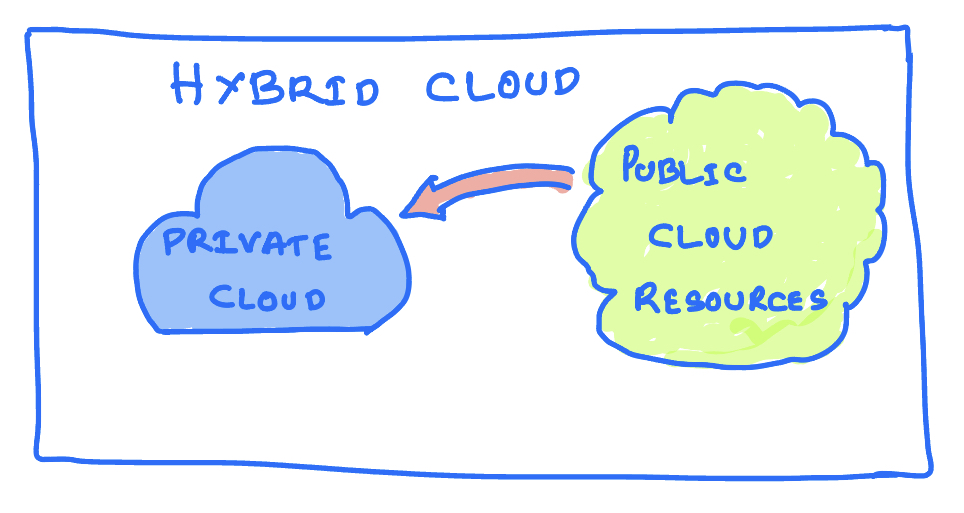
\includegraphics[scale=0.20]{/LaTeX/Notes Templates/Document/Images/hybrid.jpg}
        \end{figure}
    \end{mylist2}
    \item Multi Cloud
    \begin{mylist2}
        \item Multiple cloud providers are used.
    \end{mylist2}
    \item Azure Arc
    \begin{mylist2}
        \item Azure arc is a set of technologies helps to mange cloud environment.
    \end{mylist2}
\end{mylist1}
\section{Describe Benefits of Cloud Computing}
\chapter{Describe Azure Architecture and Services}
\section{XYZ}
\chapter{Describe Azure Management and Governance}
\section{XYZ}
\end{document}